To test GPT-3 on another task that is somewhat unusual relative to the typical distribution of text, we collected a set of 374 ``SAT analogy'' problems \cite{DBLP:journals/corr/cs-CL-0309035}.  Analogies are a style of multiple choice question that constituted a section of the SAT college entrance exam before 2005.  A typical example is ``audacious is to boldness as (a) sanctimonious is to hypocrisy, (b) anonymous is to identity, (c) remorseful is to misdeed, (d) deleterious is to result, (e) impressionable is to temptation''.  The student is expected to choose which of the five word pairs has the same relationship as the original word pair; in this example the answer is ``sanctimonious is to hypocrisy''.  On this task GPT-3 achieves 65.2\% in the few-shot setting, 59.1\% in the one-shot setting, and 53.7\% in the zero-shot setting, whereas the average score among college applicants was 57\% \cite{DBLP:journals/corr/abs-cs-0508103}  (random guessing yields 20\%).  As shown in Figure \ref{graph:sat}, the results improve with scale, with the the full 175 billion model improving by over 10\% compared to the 13 billion parameter model.

\begin{figure}
\centering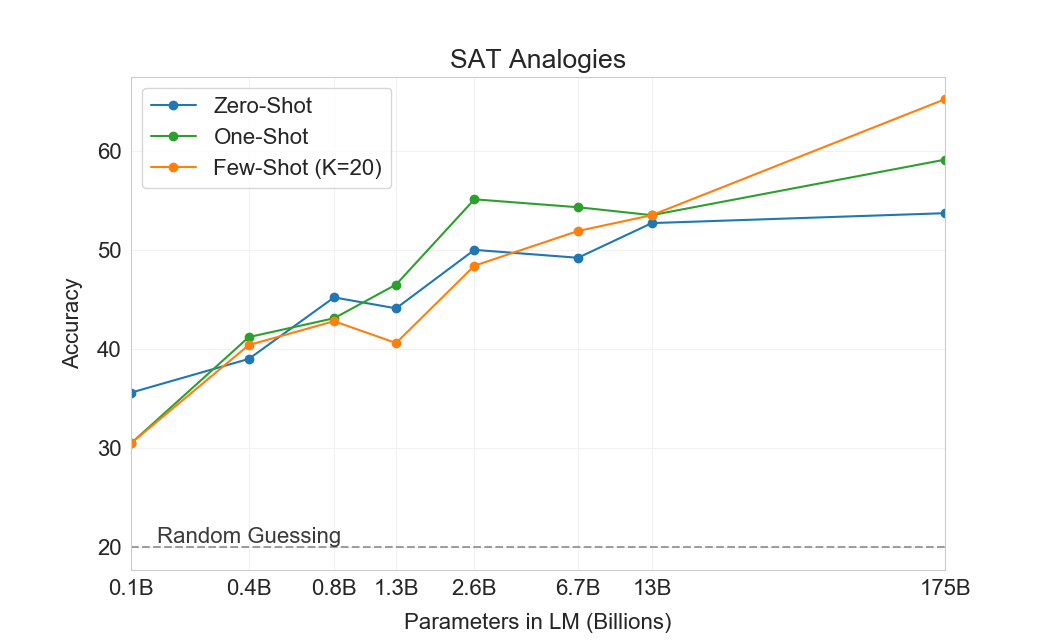
\includegraphics[width=0.8\linewidth]{graphs/scale_plots/sat_analogies.png}
\caption{Zero-, one-,and few-shot performance on SAT analogy tasks, for different sizes of model.  The largest model achieves 65\% accuracy in the few-shot setting, and also demonstrates significant gains to in-context learning which are not present in smaller models.}
\label{graph:sat}
\end{figure}